\section{Discusi\'on}

\subsection{Convergencia de PageRank}
Es importante notar que para distintos tamaños de redes las iteraciones que toma para converger son muy parecidas para el mismo c. Acá solo mostramos dos ejemplos (uno grande y uno chico) pero probamos otros casos y nos dió lo mismo. \\
Así como es lo mismo para distintas redes (fijando el c), es notable como para C chicos las iteraciones son pocas, sin embargo, el crecimiento es exponencial (o más a veces) en relación al crecimiento del c. Aquí nos referimos a la cantidad de veces que realizamos el método de la potencia.

\subsection{Convergencia de HITS}
En todos los casos podemos observar que tanto el vector de hubs como el de autoridades convergen de forma muy similar, sólo en la instancia grande hay una pequeña diferencia pero es bastante despreciable. 
Por otro lado podemos ver que los casos en los que mas drásitca es la convergencia (abortion y genetic) los valores inciales de la norma manhattan son muy altos (alrrededor de 100), provocando asi que se equiparen con las que comienzan en valores mas bajos pero convergen mas lentamente (movies y standford).
En estos dos últimos casos además podemos notar grandes saltos de convergencia pasando en pocas iteracion de 1$e^{20}$ a menos de 1$e^{80}$, entiendiendo, aca sí, que la diferencia es totalmente despreciable y el valor obtenido ya ha convergido. De todas formas consideramos que puede ser un punto de interés para analizar mas en profundidad ya que más allá de decir que entendemos de eso, no sabríamos explicar porque se produce ese salto. 

\subsection{Comparación de Tiempos}
Tanto en PageRank como en Hits notamos tiempos parecidos para instancias chicas pero a medida que crece la cantidad de nodos, el tiempo de Hits crece en forma significativa en comparación a PageRank. Esto no significa que PageRank no esté creciendo pero lo hace en menor medida que Hits y parece notar un tiempo más estable en la cantidad de nodos.


\subsection{Comparación de Calidad}

\subsection{HITS}


\subsection{Ejemplos de comportamiento esperado}

A continuación veremos en redes pequeñas como se comporta cada algoritmo para ver si su comportamiento es el esperado.

\subsubsection{PageRank}
Para mostrar un ejemplo del comportamiento del PageRank generamos una red de 11 nodos y lo corrimos con un $c$ = 0.85.

 \begin{figure}[!htb]
\begin{center}
    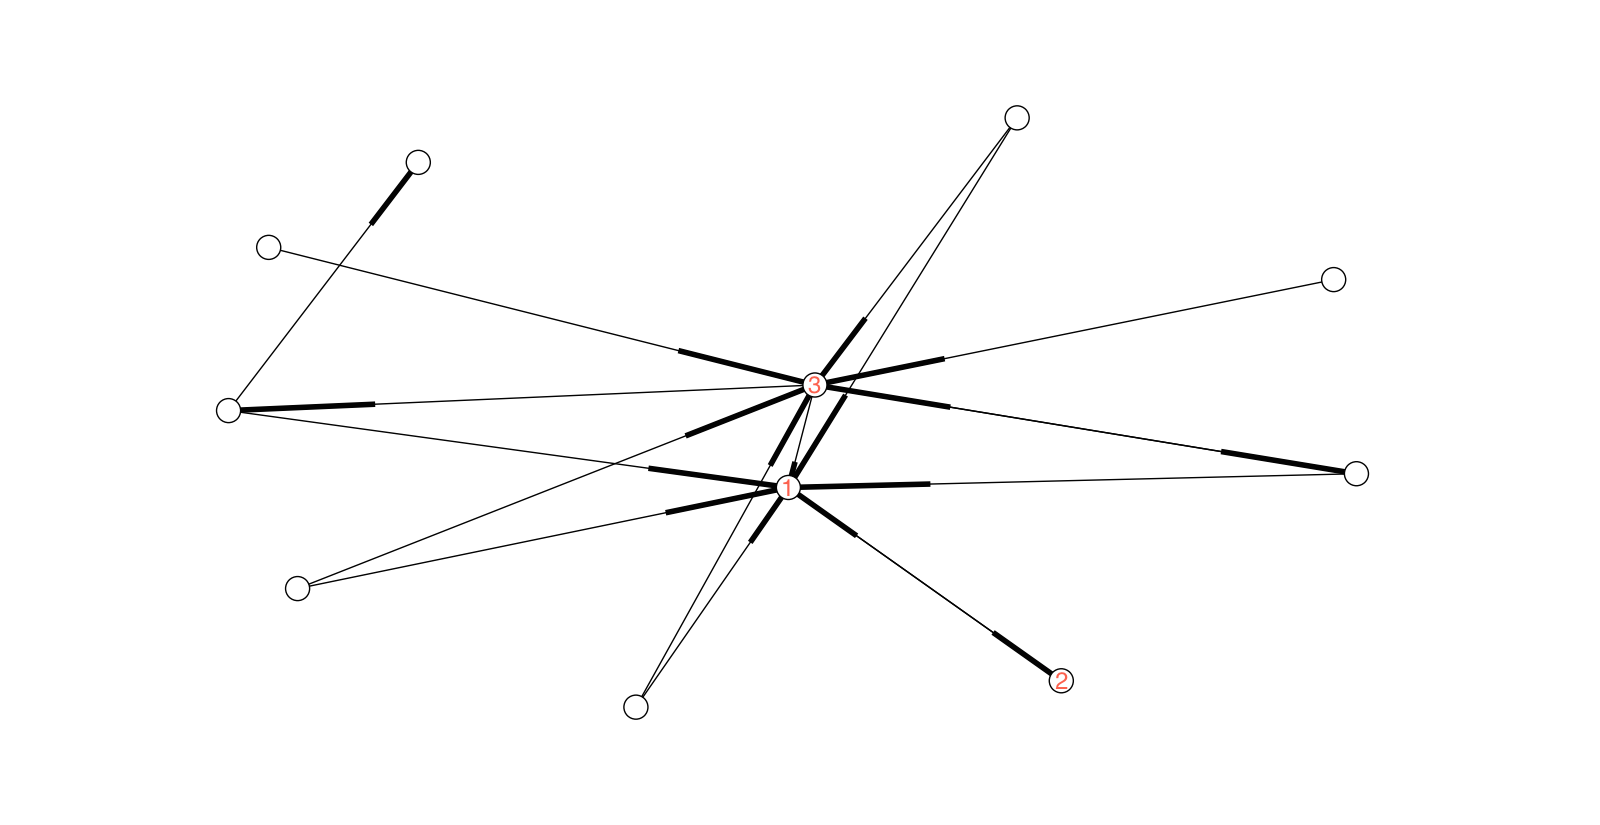
\includegraphics[scale=0.5]{imagenes/test5.png}
    \caption{Red de 11 nodos, c=0.85}
    \end{center}
\end{figure}

Lo particular de esta red es que uno $ingenuamente$ podría pensar que los dos sitios centrales 1 y 3 van a ser los que mas PageRank obtengan, pero esa suposición se basaría en que el algoritmo solo tiene en cuenta los grados de entrada de cada nodo. 
El resultado real que se obtiene de esta red es que el orden de PageRank se da por el 1, 2 y 3 (los demás nodos no son importantes para ilustrar el comportamiento). El nodo 2 le gana al 3 ya que la diferencia sustancial es que el 1 que tiene un alto valor lo apunta únicamente al 2, es decir, le da todo el peso que él tiene, mientras que el nodo 3 a pesar de tener muchos sitios que lo apuntan estos son sitios de muy bajo valor de los cuales solo tiene nodos de salida.

\subsubsection{HITS}

Dada la siguiente red, veamos que nos devuelve HITS:

 \begin{figure}[!htb]
\begin{center}
    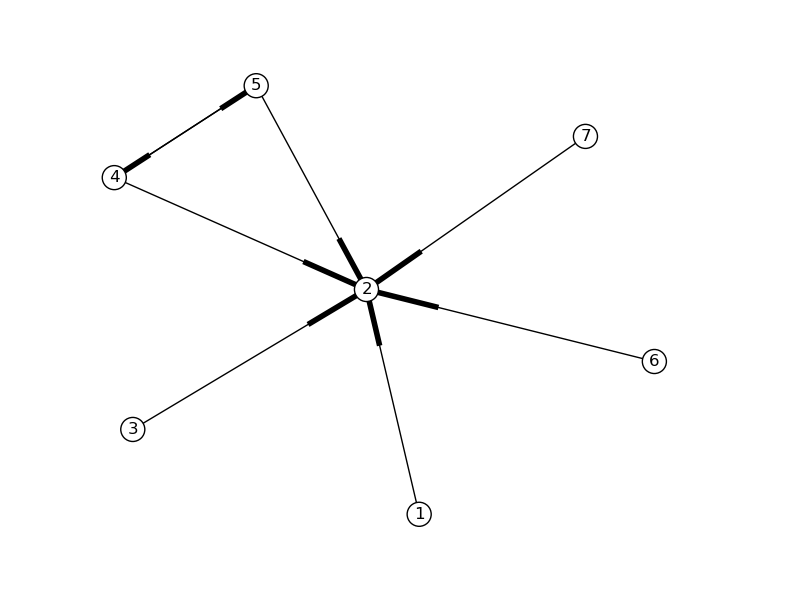
\includegraphics[scale=0.5]{imagenes/test4.png}
    \caption{Red de 7 nodos}
    \end{center}
\end{figure}

Resultado obtenido:
   $$ 
\begin{bmatrix}
              &    Autoridad  &  Hub \\
 Nodo 1 &   0.000000    &      0.383092       \\
 Nodo 2   &  0.967054    &  0.000000     \\
 Nodo 3   &  0.000000   &     0.383092  \\
 Nodo 4   &  0.180008    &     0.454401       \\
 Nodo 5   &  0.180008    &     0.454401        \\
 Nodo 6   &  0.000000    &      0.383092     \\
 Nodo 7   &  0.000000   &     0.383092 \\
\end{bmatrix} 
$$

Efectivamente podemos observar que en la columna de autoridades el nodo 2 es el mayor ya que es el que mas apuntado esta y todos aquellos que tienen 0 es porque no son apuntados por ninguno. Por otro lado en la columna de hubs podemos ver que los nodos 4 y 5 son los que mayor valor tienen ya que son los que mas apuntan a otros nodos con 2 salidas.

\subsubsection{Indeg}
 	Veamos el comportamiento dada esa pequeña red.

 	Resultado obtenido:
   $$ 
\begin{bmatrix}
              &    Puntaje \\
 Nodo 1 &    0.000000 \\
 Nodo 2   &  0.714285 \\
 Nodo 3   &  0.000000 \\
 Nodo 4   &  0.142857 \\
 Nodo 5   &  0.142857 \\
 Nodo 6   &  0.000000 \\
 Nodo 7   &  0.000000 \\
\end{bmatrix} 
$$

Este algoritmo naive es bastante claro de interpretar, y el resultado es claramente el esperado. El nodo 2 posee mucha más calidad de sitio ya que es el más apuntado, y en el segundo puesto empatando el nodo 4 y 5, por ser aquellos con más sitios apuntándolos, excpetuando el nodo 2. El resto de los nodos no reciben ningún tipo de link hacia ellos, por lo que su puntaje es de cero.

\subsection{Análisis cualitativo}

En esta sección procederemos a discutir sobre la calidad de resultados que obtenemos de cada algoritmo y luego los compararemos entre si.\\
Como el objetivo de este trabajo práctico esta enfocado al ranking web que se le asigna a los distintos sitios de internet, consideramos como buenos resultados aquellos que aparecerían en la primer página de los buscadores, es decir, los primero 10 resultados serán los que consideraremos para el análisis.

\subsubsection{PageRank}
Según el paper de Bryan y Leise, quienes proponen el algoritmo, lo más común es que el valor del navegante aleatorio sea de 0.15. Por lo tanto creemos que con este valor es donde aparecerán los mejores resultados, pero también veremos que sucede con valores de 0.5 y 0.85, ya que estos valores indican por un lado que la probabilidad del navegante entre quedarse e irse es equiprobable y por otro lado es el inverso de lo que ellos consideran como el valor más común. En valores de 0 y 1 no tendrían sentido el análisis ya que por un lado daría la matriz original y por el otro una matriz equiprobable.\\
El caso de prueba que utilizaremos es el dado por la cátedra, \textbf{Abortion}, y lo elegimos ya que es un tema bastante discutido donde se pueden encontrar resultados interesantes.


\paragraph{Resultados con un c=0.15}
\begin{enumerate}
\item
 \textbf{No relacionado con el tema}\\
http://www.allexperts.com/about.asp\\
AllExperts.com
\item
http://www.nrlc.org\\
National Right to Life Organization
\item
\textbf{No relacionado con el tema}\\
http://www.phone-soft.com/at/cyber-world/international/o1480i.htm\\
PHONE-SOFT INTERNET DIRECTORY INTERNATIONAL:HERB THERAPY LINKS
\item

http://www.lm.com/~jdehullu\\
Ariadne's Thread: On abortion, affirmative action, hate speech
\item


http://www.plannedparenthood.org\\
Planned Parenthood Federation of America
\item

http://www.gynpages.com\\
Abortion Clinics OnLine
\item

http://www.care-net.org/link.htm\\
CareNet Links
\item

http://www.naral.org\\
NARAL: Abortion and Reproductive Rights: Choice For Women
 \item

http://www.crosswalk.com/ftr/1,,17,00.htm \\
Crosswalk.com Forums - Welcome
 \item

http://www.cais.com/agm/main\\
The Abortion Rights Activist Home Page

\end{enumerate}

\paragraph{Resultados con un c=0.5}
 \begin{enumerate}
 \item http://www.allexperts.com/about.asp\\
AllExperts.com
 \item http://www.nrlc.org\\
National Right to Life Organization
 \item \textbf{No relacionado con el tema}\\
 http://home.about.com\\
About - The Human Internet
 \item \textbf{No relacionado con el tema}\\
http://www.phone-soft.com/at/cyber-world/international/o1480i.htm\\
PHONE-SOFT INTERNET DIRECTORY INTERNATIONAL:HERB THERAPY LINKS
 \item http://www.lm.com/~jdehullu\\
Ariadne's Thread: On abortion, affirmative action, hate speech
 \item http://www.plannedparenthood.org\\
Planned Parenthood Federation of America
 \item http://www.care-net.org/link.htm\\
CareNet Links
 \item http://www.gynpages.com\\
Abortion Clinics OnLine
 \item http://www.marchforlife.org\\
The March For Life Fund Home Page
 \item \textbf{No relacionado con el tema}\\
http://www.jbs.org\\
The John Birch Society
 \end{enumerate}
 
\paragraph{Resultados con un c=0.85}
 \begin{enumerate}

 \item 
 \textbf{No relacionado con el tema}\\
 http://www.jbs.org\\
The John Birch Society
 \item 
 \textbf{No relacionado con el tema}\\
http://home.about.com\\
About - The Human Internet
 \item 
 \textbf{No relacionado con el tema}\\
http://www.allexperts.com/about.asp\\
AllExperts.com
 \item
  \textbf{No relacionado con el tema}\\
http://www.aobs-store.com\\
American Opinion Book Services Online Store
 \item
http://www.nrlc.org\\
National Right to Life Organization
 \item 
 \textbf{No relacionado con el tema}\\
http://www.trimonline.org\\
TRIMonline - Lower Taxes Through Less Government
 \item
http://www.marchforlife.org\\
The March For Life Fund Home Page
 \item 
 \textbf{No relacionado con el tema}\\
http://www.phone-soft.com/at/cyber-world/international/o1480i.htm\\
PHONE-SOFT INTERNET DIRECTORY INTERNATIONAL:HERB THERAPY LINKS
 \item 
\textbf{No relacionado con el tema}\\
http://www.reagan.com\\
The Reagan Information Interchange
 \item 
 \textbf{No relacionado con el tema}\\
http://www.pregnancycenters.org\\
Pregnancy Centers Online
 \end{enumerate}

En base a los resultados se puede ver como a medida que aumenta el $c$ empiezan a aparecer resultados que poco tienen que ver con el tema directamente, ya que puede estar relacionado de alguna forma o no diferenciarse tanto del eje temático.\\
Nos pareció extraño que aparece siempre muy bien posicionado el sitio web All Experts, que nada tiene que ver con el tema de los abortos, por lo tanto decidimos hacer un foco especial en este para ver porque sucedía esto y llegamos a la conclusión que es debido a que el factor mas determinante es que gran cantidad de sitios referidos al tema y a su vez bien posicionados (aunque fuera del top 10) apuntaban al mismo, y por lo tanto le daban bastante peso a All Experts.\\
Sucede algo parecido con otro sitio de venta de software que aparece pero no nos pareció importante su análisis ya que es un claro caso de publicidad paga en anuncios de los sitios que hablan sobre el tema.\\
Aunque se pueda ver que con un $c$ menor los resultados tienen relación con el tema nos pareció que no son lo suficiente buenos como para considerarlos excelente resultados cuando se busca sobre un tema tan discutido como el aborto, esperando quizás más definiciones sobre el tema y luchas por su legalización/penalización. 

\subsubsection{HITS}
Este analásis de calidad lo haremos sobre el tema death penalty. Veremos cuales son los primeros 5 resultados que devuelve HITS en cuanto a autoridades y hubs.

\paragraph{Resultados Hubs}
\begin{enumerate}
\item
http://www.clarkprosecutor.org/html/links/dplinks.htm\\
Death Penalty Links
\item
http://faculty.etsu.edu/blankenm/deathlinks.htm\\
Death Penalty Links
\item
http://coramnobis.com/portal/deathpen.html\\
A Capital Defender's Toolbox: criminal defense  death penalty litigation online resource center
\item
http://info-s.com/deathpenalty.html\\
The Info Service
\item
http://members.xoom.com/ccadp/links.htm\\
Canadian Coalition Against the Death Penalty - Collection of Links


\end{enumerate}

\paragraph{Resultados Autoridades}
\begin{enumerate}
\item
http://sun.soci.niu.edu/~critcrim/dp/dp.html\\
Death Penalty Information
\item
http://www.aclu.org/issues/death/hmdp.html\\
Death Penalty and the ACLU
\item
http://www.ncadp.org\\
National Coalition To Abolish the Death Penalty
\item
http://www.smu.edu/~deathpen\\
Death Penalty News and Updates
\item
http://www.deathpenalty.org\\
Death Penalty Focus


\end{enumerate}

Aquí podemos observar claramente que la calidad además de ser, a priori, buena y correcta, tiene coherencia. La mayoría de los hubs sobre el tema son conjunto de links sobre pena de muerte, servicios de información o 
central de recursos sobre litigios en penas de muerte. Por otro lado, las autoridades son diarios con noticias y novedades, organizaciones enfocadas a eso o páginas institucionales (.edu). Ambos tienen sentido en sus 
categorías ya que es totalmente lógico que páginas institucionales sean fuentes propias de información que son citadas por otras (osea autoridades) o que una central de recursos linkee a muchos otros citios (osea un hub).\\
También es de destacar que ningún link pareciera ser spam, o sobre algo no relacionado.

\subsubsection{Comparación}

Si comparamos los resultados del PageRank con un $C$ alto claramente da mejores respuestas el HITS. Sin embargo en el paper de Bryan y Leise$[3]$ se recomienda un $C$ de 0.15, con este valor los resultados mejoran notoriamente aunque sigue habiendo algunos que no corresponden o son SPAM. 
Teniendo en cuenta estas pruebas HITS parecería ser el mejor, aunque no podemos asegurarlo ya que no hicimos las suficientes pruebas y tenemos la cuestión de que PageRank esta pensado para grandes escalas en constante crecimiento, por lo que tendríamos que tener en cuenta eso también a la hora de probarlo rigurosamente.
